\chapter{DSP introduction}
This chapter will give a general introduction to the TMS320C5515 DSP and its programming languages C, assembler and how they function together. An overview of the TMS320C55xx architecture can be seen on \autoref{fig:DSP}. It has four different processing units in the CPU, the instrution buffer unit (UI), the program flow unit (PU), the adress-data flow unit (AU) and the data computation unit (UI) connected to 12 different adress and databusses.  
 
\begin{figure}[H]
\centering
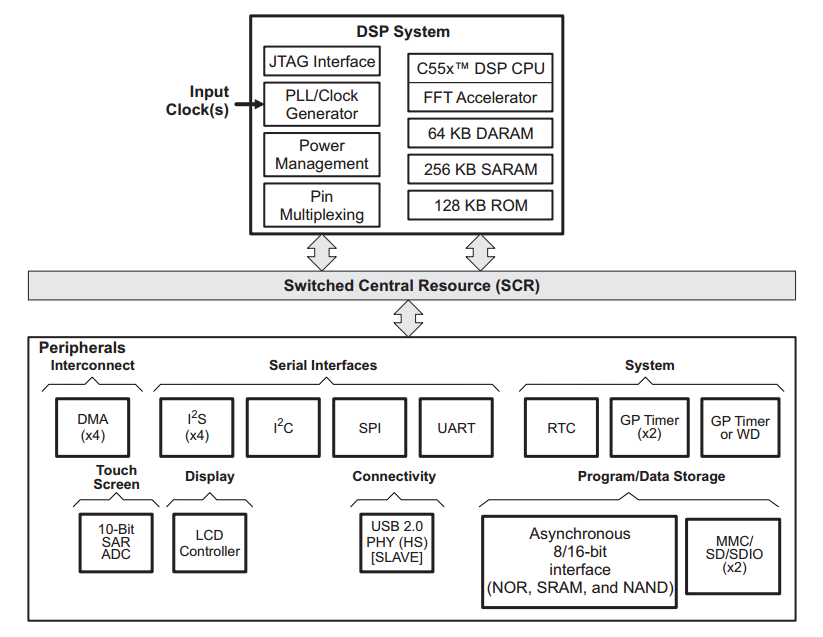
\includegraphics[width=\textwidth]{cpuCore.png}
\label{fig:DSP}
\caption{Functionel block diagram of the DSP.}
\end{figure}
\todo[inline]{http://www.ti.com/lit/ug/sprufp0c/sprufp0c.pdf    -    TMS320VC5505 DSP System User's Guide}

The CPU has a harvard strucure which means that data and program memory is seperate. This has the advantage that program and data can fetched and decoded in parallel. 

DSP
Assembler
Instruction set
C
C compiler 
